%\documentclass[onecolumn, 12pt]{book}
%
%\usepackage[latin1]{inputenc}   
%\usepackage{amsmath}
%\usepackage{algorithm}
%\usepackage{algorithmic} 
%%\usepackage[T1]{fontenc}
%
%%\usepackage[francais]{babel}     
%\usepackage{layout}    
%\usepackage[top=2cm, bottom=2cm, left=2cm, right=2cm]{geometry} 
%\usepackage{setspace}
%\usepackage{soul}
%\usepackage{color} 
%\usepackage{verbatim}
%\usepackage{moreverb}
%\usepackage{listings}
%\usepackage{url}
%\usepackage{graphicx}
%\usepackage[outdir=./]{epstopdf}
%\usepackage{caption}
%\usepackage{setspace}
%\usepackage{amssymb} % used for not exists symbol ==> \nexists
%\usepackage{amsthm}
% 
%\title{chapitre3: les graphes adjoints ou line graphes}
%\author{Wilfried Ehounou}
%\date{\oldstylenums{\today}} 
%
%\newtheorem{definition}{D\'efinition}
%\newtheorem{property}{Propri\'et\'e}
%\newtheorem{theorem}{Th\'eor\`eme}
%\newtheorem{claim}[theorem]{Claim}
%\newtheorem{proposition}[theorem]{Proposition}
%\newtheorem{lemma}[theorem]{Lemme}
%\newtheorem{corollary}[theorem]{Corollaire}
%\newtheorem{conjecture}[theorem]{Conjecture}
%\newtheorem{observation}{Observation}
%\newtheorem{example}{Exemple}
%\newtheorem{remark}{Remarque}
%
%%---insert paragraph (use 4) and subparagraph (use 5) to table of contents
%%\setcounter{tocdepth}{4} 
%%\setcounter{secnumdepth}{4}
%
%%---- path figures ----
%\graphicspath{{/home/willy/Documents/courbePython/courbeDegreCoutMinAleatoire_11_09_2017/}
%{/home/willy/Documents/courbePython/courbeDegreCoutMinAleatoire_11_10_2017/}
%{/home/willy/Documents/courbePython/courbeDegreCoutMinAleatoire_11_09_2017/comparaison_MethodesCorrection_fctDeCout_permut_aleatoire_coutMin_degreMin/}
%{/home/willy/Documents/latexDoc/redactionThese/fusion_fichiers/images_fusionChapitres/}}
% 
%\begin{document}

Soit la  matrice de corr\'elation $M_{c}$ d\'esignant les probabilit\'es de corr\'elation entre les arcs d'un graphe $G$. 
Chaque case de la matrice $M_c$ d\'efinit le pourcentage de corr\'elation entre deux arcs. Une corr\'elation, proche de $1$, indique que les arcs partagent un sommet tandis qu'une valeur, qui tend vers $0$, signifie qu'il existe aucun sommet en commun entre ces arcs.

\subsubsection{Erreurs de corr\'elation}
Dans la figure \ref{reseauElectriqueMatriceCorrelation}, les arcs $a_2$ et $a_3$ partagent le sommet d'extr\'emit\'e initiale et leur valeur de corr\'elation est de $0.85$.  De m\^eme, il n'existe aucun sommet commun aux arcs $a_1$ et $a_6$ impliquant que leur corr\'elation tend vers $0$ (corr\'elation \'egale \`a $0.21$). 
Toutefois, certains arcs n'ayant aucun sommet en commun, ont des valeurs de corr\'elations tr\`es \'el\'ev\'es (proche de $1$). 
C'est le cas des arcs $a_5$ et $a_7$ dont leur valeur de corr\'elation est de $0.89$ (figure \ref{reseauElectriqueMatriceCorrelation}.b).
\newline
Ce type de corr\'elations, appel\'e {\em erreurs de corr\'elation}, est d\^u aux lissages des signaux \'electriques caus\'es par la pr\'esence d'onduleurs ou des \'equipements, dans des branches diff\'erentes, ont des profils de consommation identiques sur la p\'eriode de temps. En g\'en\'eral, ces profils de consommation sont quasi-constants avec des variations tr\`es faibles.
\begin{centering}\vspace{-0.5em}
	\begin{figure}[htb!]\vspace{-0.5em}
	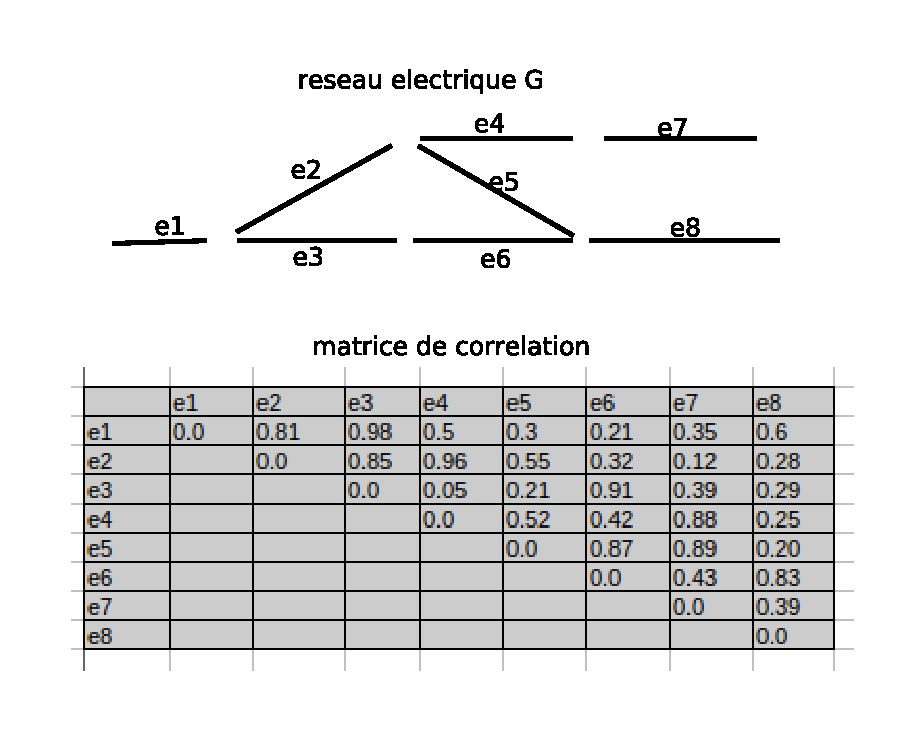
\includegraphics[scale=0.50]{reseauElectriqueMatriceCorrelation.eps}\vspace{-0.5em}
	\caption{ Le r\'eseau \'electrique $G$ et sa matrice de corr\'elation $M_c$. a) r\'eseau \'electrique, b) matrice de corr\'elation associ\'ee. Les cases en jaunes et en rouges sont les corr\'elations erron\'ees. }\vspace{-0.5em}
	\label{reseauElectriqueMatriceCorrelation}
	\end{figure}
\end{centering}

\subsubsection{Matrice de corr\'elation : un graphe adjoint}
Soient la valeur de seuil $s$ et la matrice de corr\'elation $M_{c,s}$ appliqu\'ee avec ce seuil.
Cette matrice $M_{c,s}$ est binaire avec $0$ et $1$ d\'esignant respectivement aucune corr\'elation entre arcs (dont pas de sommets en commun) et l'existance d'un sommet entre ces arcs.
\newline
Chaque arc peut \^etre repr\'esent\'e par un sommet et deux arcs ayant un sommet en commun (quelque soit son extr\'emit\'e) ont leurs sommets respectifs adjacents. 
Cela implique que la matrice $M_{c,s}$ peut \^etre consider\'ee comme la matrice d'adjacence d'un graphe adjoint et ce graphe adjoint est celui sous-jacent au graphe non orient\'e du r\'eseau \'electrique $G$. 
\newline
Dans la litt\'erature, le graphe adjoint est design\'e par {\em linegraph}. Nous utilisons {\em line graphe} dans la suite du document pour indiquer un graphe adjoint.

\begin{definition}  Line graphe \newline
Soit un graphe non orient\'e $G$.
Le line graphe $H$ d'un graphe $G$ est un graphe dont chaque sommet correspond \`a une ar\^ete de $G$ et deux sommets de $H$ sont adjacents si et seulement si leurs ar\^etes respectives dans $G$ ont un sommet en commun. \newline
Avec $G$ ayant $n$ sommets et $m$ ar\^etes, le graphe $H$ a $m$ sommets et $E$ ar\^etes dont 
$$ E = \sum_{i=1 }^{n} d_i(d_i -1)/2$$, 
$d_i$ \'etant le degr\'e de chaque sommet $i$ de $G$.
\end{definition}
Le graphe $G$ est  appel\'e le {\em graphe racine} de $H$. 
Un exemple de graphe racine et son line graphe est present\'e dans la figure \ref{rootGrapheLineGrapheExemple}
\begin{centering}\vspace{-0.5em}
	\begin{figure}[htb!]\vspace{-0.5em}
	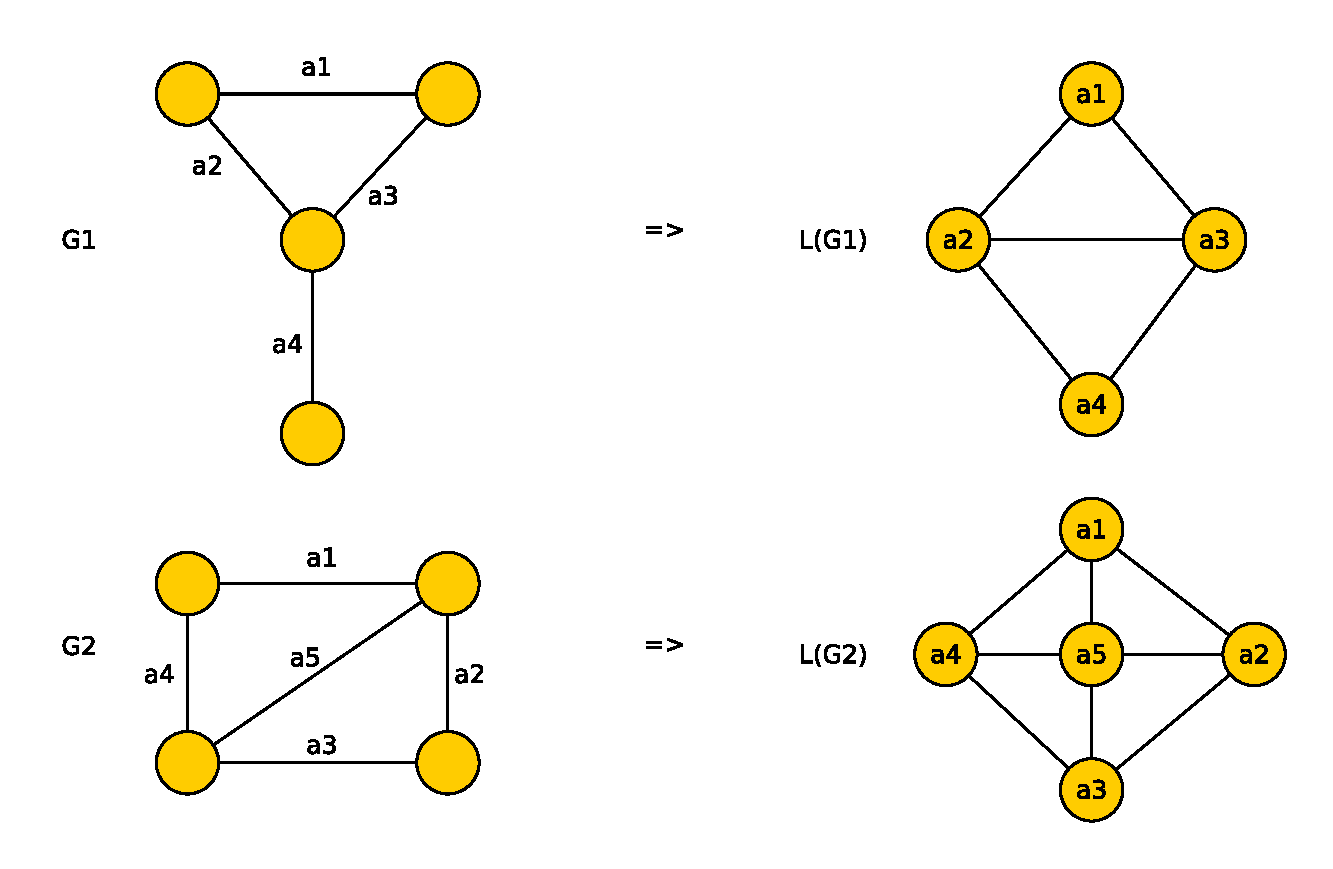
\includegraphics[scale=0.50]{rootGrapheLineGrapheExemple.eps}\vspace{-0.5em}
	\caption{ Le graphe racine $G$ et son line graphe L(G) }\vspace{-0.5em}
	\label{rootGrapheLineGrapheExemple}
	\end{figure}
\end{centering}
\newline
Ce concept a \'et\'e introduit par {\em Whitney} \cite{isomorphismeLineGraphe} qui montra que l'isomorphisme des ar\^etes implique l'isomorphisme pour des graphes connexes \`a l'exception des graphes $K_3$ (graphe triangle) et $K_{1,3}$ (graphe \'etoile). 
\begin{theorem}
\label{grapheIsomorphismeEnAretes}
Si deux line graphes $L(G_1)$ et $L(G_2)$ sont isomorphes et connexes alors leurs graphes racines $G_1$ et $G_2$ sont aussi isomorphes sauf si $G_1 = K_3$ et $G_2 = K_{1,3}$.
\end{theorem}

% caracteristique d'un line graphe
\begin{proposition}
Le graphe \'etoile $K_{1,3}$ n'est pas un {\em line graphe}.
\end{proposition}
\begin{proof}
Supposons que $K_{1,3}$ est le line graphe de $H$ ($K_{1,3} = L(H)$). 
Alors $H$ est un graphe connexe de quatre ar\^etes.
Tous les graphes connexes de quatres ar\^etes sont repr\'esent\'es dans la figure  \ref{graphesRacinesDeQuatresAretes}. 
Comme $L(C_4) = C_4$ par le th\'eor\`eme \ref{grapheIsomorphismeEnAretes} et $L(K_{1,3} + e) = K_4 + e$ (voir figure \ref{rootGrapheLineGrapheExemple}), $L(H)$ ne peut \^etre que l'un des trois arbres $P_4$, $K_{3,2}$ et $K_{1,4}$.
Ce qui est contraire \`a notre hypoth\`ese de d\'epart ($K_{1,3} = L(H)$).
\end{proof}
\begin{centering}\vspace{-0.5em}
	\begin{figure}[htb!]\vspace{-0.5em}
	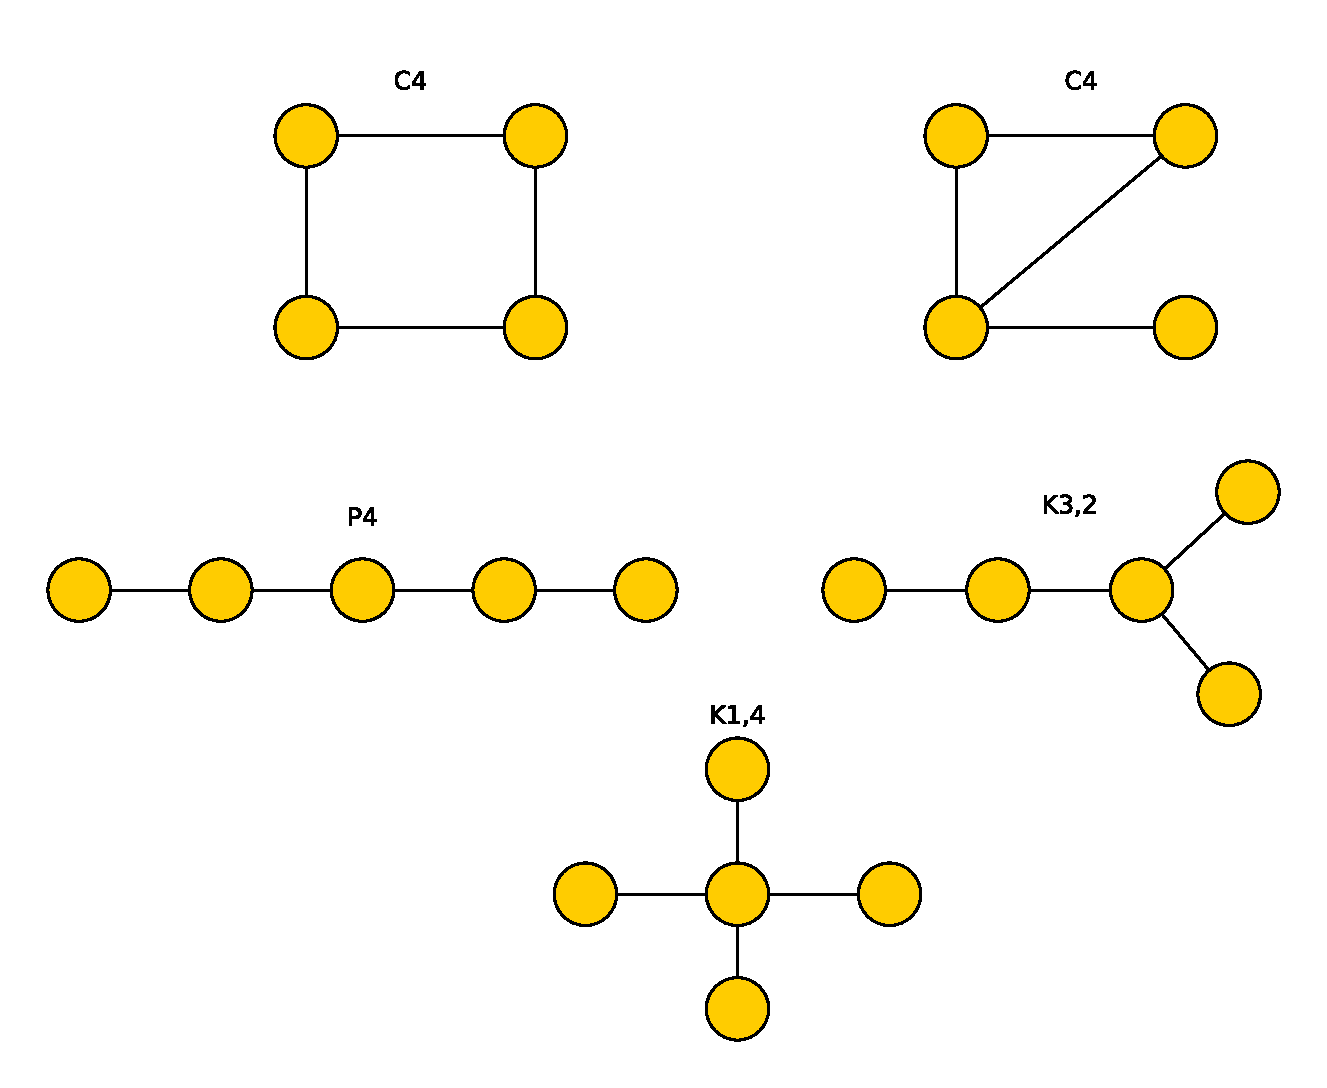
\includegraphics[scale=0.50]{graphesRacinesDeQuatresAretes.eps}\vspace{-0.5em}
	\caption{ Les graphes racines possibles de $K_{1,3}$ de quatres ar\^etes   }\vspace{-0.5em}
	\label{graphesRacinesDeQuatresAretes}
	\end{figure}
\end{centering}

Beineke et Hemminger \cite{neufLineGrapheInterdit}  affichent les neufs sous-graphes ne pouvant pas avoir de line graphes.
\begin{theorem}
Aucun des neufs sous-graphes de la figure \ref{neufSousGraphesInterditDesLineGraphes} ne peut \^etre un sous graphe d'un line graphe $G$.
\end{theorem}
\begin{centering}\vspace{-0.5em}
	\begin{figure}[htb!]\vspace{-0.5em}
	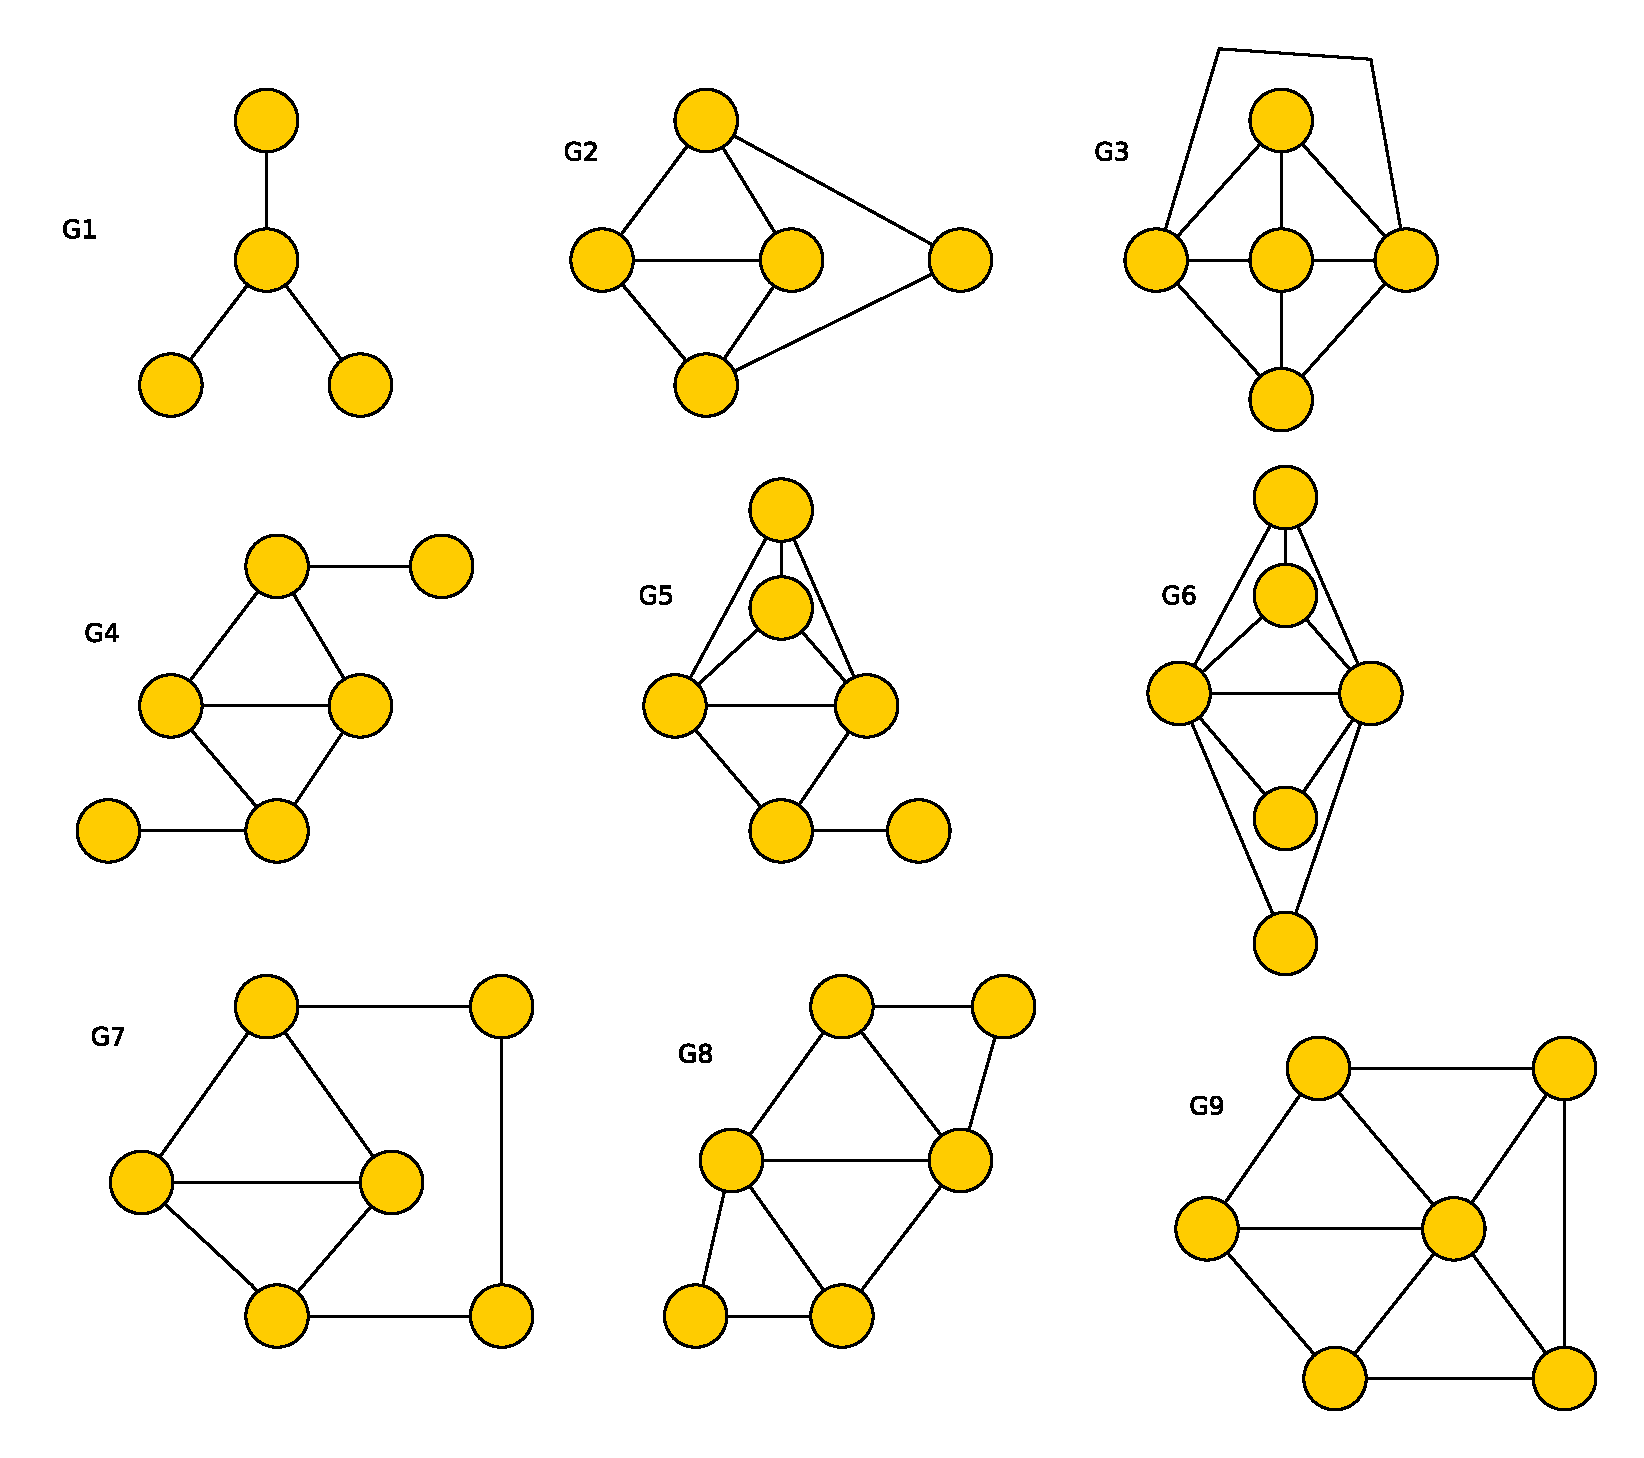
\includegraphics[scale=0.50]{neufSousGraphesInterditDesLineGraphes.eps}\vspace{-0.5em}
	\caption{ Line graphes et sous graphes interdits }\vspace{-0.5em}
	\label{neufSousGraphesInterditDesLineGraphes}
	\end{figure}
\end{centering}

\begin{theorem}
Les ar\^etes d'un line graphe $G$ sont partitionn\'ees en sous graphes complets (Cliques) de tel sorte que chaque ar\^ete ne peut appartenir qu'\`a un seul sous graphe.
%\newline
%a graph ....... generaledLineGraph.pdf theorem 1
\end{theorem}
\begin{proof}
Soit $G$ le line graphe de $H$. \newline
* de line graphe \`a des sous graphes :
nous supposons que $H$ est connexe.
Alors les ar\^etes dans le graphe \'etoile de chaque sommet de $H$ induit un clique dans $G$. Et chaque ar\^ete de de $G$ est couverte par exactement une clique. 
Pour chaque arete de $H$ appartenant \`a deux graphes \'etoiles de deux sommets de $H$, aucun sommet de $G$ est contenu dans plus de deux cliques. \newline
** de sous graphes \`a un line graphe:
\'etant donn\'e une d\'ecomposition des ar\^etes de $G$ en cliques $C_1, C_2,\cdots, C_n$ satisfaisant le th\'eor\`eme ci dessus, nous construisons le graphe $H$ dont le line graphe est $G$.
Les sommets de $H$ correspondent \`a l'ensemble $C$ de cliques de la d\'ecomposition   avec l'ensemble $U$ de sommets de $G$ appartenant \`a une clique $C_i$ uniquement.
Alors $C \cup U$ est l'ensemble de sommets de $H$ et deux de ses sommets sont adjacents s'il y a une intersection non vide. Alors $H$ est un graphe d'intersection $\Omega(C \cup U)$.
\end{proof}

% related works sur les reconstructions de topologie
Divers travaux existent dans la reconnaissance de line graphes et son graphe racine associ\'e.
\newline
Le premier algorithme propos\'e est celui de LEHOT \cite{decompositionEnCliquesParArcs}. Il utilise la propri\'et\'e d\'efinie par VAN ROOIJ and WILF \cite{ROOIJetWILF1965interchange} \'enoncant qu'un graphe $G$ est un line graphe si $G$ ne contient pas de sous graphe induit $K_{1,3}$ and si deux graphes triangles ``Odd'' ont une ar\^ete commune, le sous graphe induit par ces sommets est une clique $K_4$.
Son algorithme n'effectue que la reconnaissance de line graphe et la complexit\'e est en $O(n) + E$ avec $n$ le nombre de sommets de $G$ et $E$ le nombre d'ar\^etes de $L(G)$.
Rappelons qu'une graphe triangle $\{a_1,a_2,a_3\} \subseteq V(L(G))$ est ``Odd'' s'il existe un sommet $e \in V(G)$ incident \`a  au moins un des sommets $\{a_1, a_2, a_3\}$. Ce triangle est ``Even'' dans le cas contraire. 
% def triangle ODD/EVEN 
% A triangle {e1,e2,e3}⊆V(LG) is said to be an odd triangle if there exists a vertex e∈V(G) incident to exactly one or all of {e1,e2,e3}, and it is said to be even otherwise.
% http://doc.sagemath.org/html/en/reference/graphs/sage/graphs/line_graph.html
\newline
L'algorithme de ROUSSOPOULOS utilise une autre propri\'et\'e des line graphes provenant des travaux de KRAUSZ \cite{krausz1943demonstration}. Il affirme que $G$ est un line graphe si les ar\^etes  de  $G$ peuvent \^etre partition\'ees en cliques  de tel sorte qu'aucun sommet ne soit couvert par deux cliques. 
Cette algorithme non seulement d\'etecte si $G$ est un line graphe mais fournit son graphe racine en temps lin\'eaire $O(max(\{m,n\})$, avec $m$ et $n$ le nombre de sommets et d'ar\^etes respectivement.
\newline
Cette algorithme, bas\'e sur la preuve de ORE \cite{ORE} du th\'eor\`eme de Whitney \cite{whitney1932congruent} qui stipule que si deux graphes connexes avec plus de quatre sommets sont isomorphes en ar\^etes alors il existe exactement un isomorphisme en sommets qui induit un isomorphisme en ar\^etes.  
Propos\'e par Klauss Simon et Daniele Degiorgi \cite{decompositionEnCliques}, cette approche est une simplication du probl\`eme de reconnaissance de line graphes. Les deux pr\'ec\'edents algorithmes  utilisent les propri\'et\'es globales des line graphes tandis que celui ci utilisent uniquement les propri\'et\'es locales permettant une reconnaissance incrementale. Par ailleurs il permet de v\'erifier en temps lin\'eaire si une modification locale (i.e l'ajout et la suppression) preserve les caract\'eristiques du line graphe.
\newline
Tous les algorithmes existants se limitent \`a un r\'esultat n\'egatif lorsque le graphe $G$ n'est pas un line graphe.
Les algorithmes, que nous soumettons, retournent la d\'ecomposition en cliques de $G$ si $G$ est un line graphe ou dans le cas contraire, la d\'ecomposition du line graphe le plus proche de $G$.

%\end{document}